\documentclass{article}

\usepackage{amsmath}
\usepackage{amssymb}
\usepackage{graphics}
\usepackage{listings}
\usepackage{tcolorbox}
\usepackage{verbatim}

\DeclareMathOperator*{\argmin}{arg\,min}

\marginparwidth 0pt
\oddsidemargin  0pt
\evensidemargin  0pt
\marginparsep 0pt
\topmargin   0pt
\textwidth   6.5in
\textheight  8.5in
\setlength{\parindent}{0em}

\newtheorem{theorem}{Theorem}
\newtheorem{conjecture}{Conjecture}

\newenvironment{packed_itemize}{
\begin{itemize}
  \setlength{\itemsep}{0pt}
  \setlength{\parskip}{0pt}
  \setlength{\parsep}{0pt}
}{\end{itemize}}

\newenvironment{packed_enumerate}{
\begin{enumerate}
  \setlength{\itemsep}{1pt}
  \setlength{\parskip}{0pt}
  \setlength{\parsep}{0pt}
}{\end{enumerate}}

\definecolor{codeback}{RGB}{235,255,255}

\lstset{ %
language=Python,                % choose the language of the code
basicstyle=\footnotesize,       % the size of the fonts that are used for the code
numbers=left,                   % where to put the line-numbers
numberstyle=\footnotesize,      % the size of the fonts that are used for the line-numbers
stepnumber=1,                   % the step between two line-numbers. If it is 1 each line will be numbered
numbersep=10pt,                  % how far the line-numbers are from the code
backgroundcolor=\color{codeback},  % choose the background color. You must add \usepackage{color}
showspaces=false,               % show spaces adding particular underscores
showstringspaces=false,         % underline spaces within strings
showtabs=false,                 % show tabs within strings adding particular underscores
frame=single,           % adds a frame around the code
tabsize=2,          % sets default tabsize to 2 spaces
captionpos=b,           % sets the caption-position to bottom
breaklines=true,        % sets automatic line breaking
breakatwhitespace=false,    % sets if automatic breaks should only happen at whitespace
escapeinside={(*@}{@*)}          % if you want to add a comment within your code
}

\begin{document}

\begin{center}
  {\huge\bf
  Symbolic Calculations with sympy\\ 
  Mathematical Programming with Python\\
  }
  https://people.sc.fsu.edu/$\sim$jburkardt/classes/math1800\_2023/sympy/sympy.pdf
\end{center}

\hrule

\begin{center}
  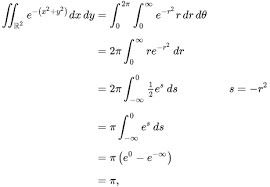
\includegraphics[scale=0.60]{gaussian_integral.png}
  \vskip 0.1in
  {\it{A tricky path integrates the Gaussian integral to a simple result.}}
\end{center}

\begin{tcolorbox}[colback=blue!5,title="The sympy library"]
{\it{
  \begin{packed_itemize}
    \item{ The {\tt{sympy}} library supports symbolic calculations;}
    \item{ Symbolic calculations work with exact data and return 
           exact results.}
    \item{ Symbolic calculations can fail to produce a usable
           result if no suitable algorithm is known.}
    \item{ {\tt{sympy}} can produce results for expressions
           in arithmetic, algebra, integration,
           limits, summation, differentiation, differential equations
           and linear algebra;}
    \item{ Results can be ``translated'' to numerical values;}
  \end{packed_itemize}
}}
\end{tcolorbox}

\section{The {\tt{sympy}} library}

The {\tt{sympy}} library carries out mathematical operations on symbolic
variables and expressions.  You are perhaps more familiar with numerical
calculations, in which variables are given finite precision numerical
values, and operated on with finite precision.  The results of such operations
are numerical, and of limited precision.  The operations carried out by
{\tt{sympy}} are intended to be mathematically exact; {\tt{sympy}} can
operate on formulas rather than numbers, and so, for instance, it can
be asked to determine the formula for the derivative of function, rather
than the value of that derivative at a specific argument.  At any time,
however, the results of {\tt{sympy}} can be evaluated at specific numerical
values.
\vskip 0.1in
Versions of {\tt{sympy}} have been used to build applications
in chemistry, circuit analysis, finite elements, linear algebra,
optimization, quantum mechanics, relativity, statistical modeling, 
and tensor algebra.
\vskip 0.1in
The {\tt{sympy}} homepage is 
\begin{verbatim}
https://docs.sympy.org/latest/index.html
\end{verbatim}
and has instructions on downloading and installing the package, as well
as a tutorial.

\section{The {\tt{sympy}} environment}

To work with the {\tt{sympy}} library, it is necessary to issue
the appropriate {\tt{import}} command.
Depending on your taste, you may import every additional
{\tt{sympy}} function with a separate statement
\begin{lstlisting}[numbers=none]
from sympy import plot
from sympy import sin
from sympy import symbols
\end{lstlisting}
which can also be rolled up into a single statement
\begin{lstlisting}[numbers=none]
from sympy import plot, sin, symbols
\end{lstlisting}
\vskip 0.1in
But if you are going to make extensive use of library
functions, it may be worthwhile to import the entire library
\begin{lstlisting}[numbers=none]
from sympy import *
\end{lstlisting}

\section{Doing simple arithmetic}

If you import the entirety of the {\tt{sympy}} library, then
you can 
\begin{lstlisting}[numbers=none]
from sympy import *
pi
pi.evalf()     # evaluate to default number of decimals
pi.evalf(30)   # evaluate to 30 decimal places
sqrt ( pi ).evalf(20)
sqrt ( 600 )
factorial(20)
binomial(100,30)
\end{lstlisting}
What is more important is that you can declare symbolic variables
and then manipulate functions of them:
\begin{lstlisting}[numbers=none]
x = symbols ( 'x' )
expr = sqrt ( 1 - cos(x)**2 )
simplify ( expr )    # sqrt(sin(x)**2), NOT sin(x)!\
poly = ( x + 7 ) * ( x**2 - 4 * x + 3 )
poly / ( x - 1 )
\end{lstlisting}
As we will see, you can do much more with symbolic expressions,
including integration, differentiation, series expansion, 
and taking limits.  

\section{Working with the humps() function}

For some of the following exercises, we will repeatedly use the
``humps()'' function to test out features of {\tt{sympy}}.  There is
nothing special about this function, except that it's not just a
boring old polynomial.  We will be interested in the function especially
over the interval $0 \leq x \leq 2$, and we want to understand how to
define it, evaluate it, plot it, compute derivatives and integrals,
request zeros and extreme values, and solve a related differential
equation. 
\vskip 0.1in
The function can be defined mathematically as:
\begin{displaymath}
y(x) = \frac{1}{(x-0.3)^2 + 0.01 } + \frac{1}{(x-0.9)^2 + 0.04} - 6
\end{displaymath} 
but we will see in a moment that we should rewrite the function to avoid
the decimal fractions.
\vskip 0.1in
Here is a plot of the function:
\begin{center}
  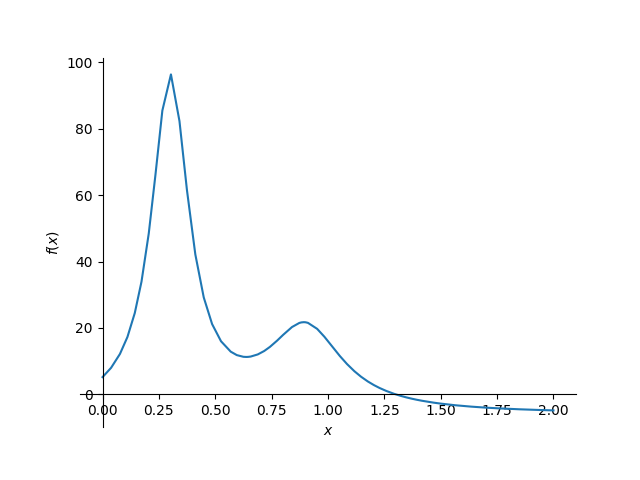
\includegraphics[scale=0.60]{humps_plot.png}
\end{center}

\section{Defining a function}

A symbolic function is simply an expression involving symbolic variables.
Our {\tt{humps()}} function only depends on a single variable $x$.  We
can define it using normal Python syntax; however, the decimal fractions
would be interpreted as limited precision real values.  To avoid this,
we multiply top and bottom of the fractions by 100 to get a form that
the symbolic package can handle better.  
\vskip 0.1in
Here is how we define humps:
\begin{lstlisting}[numbers=none]
  from sympy import symbols

  x = symbols ( 'x' )

  humps = 100 / ( ( 10 * x - 3 )**2 + 1 ) \
        + 100 / ( ( 10 * x - 9 )**2 + 4 ) \
        - 6
\end{lstlisting}

\section{Evaluating a function}

If you have defined an expression involving a symbolic variable,
then the {\tt{subs()}} operator substitutes a given symbol,
expression, or value for the symbolic variable. 
If we want to do some numerical calculations with our symbolic
function the {\tt{lambdify()}} operator will create a corresponding
numerical function for us that can be evaluated by {\tt{numpy}}:
\begin{lstlisting}[numbers=none]
  from sympy import cos
  from sympy import lambdify
  from sympy import symbols
  import numpy
  import numpy as np

  x = symbols ( 'x' )

  humps = 100 / ( ( 10 * x - 3 )**2 + 1 ) \
        + 100 / ( ( 10 * x - 9 )**2 + 4 ) \
        - 6

  y = symbols ( 'y' )
  humps_y = humps.subs ( x, y )
  print ( '  humps.subs(x,y) = ', humps_y )

  humps_cosy = humps.subs ( x, cos(y) )
  print ( '  humps.subs(x,cos(y)) = ', humps_cosy )

  humps_1 = humps.subs ( x, 1 )
  print ( '  humps.subs(x,1) = ', humps_1 )
  
  z = np.linspace ( 0.0, 2.0, 5 )
  humps_lambda = lambdify ( x, humps, 'numpy' )
  humps_lambda ( z )
  print ( '  humps(z) = ', humps_lambda ( z ) )
\end{lstlisting}

\section{Plotting a function}

We may wish to plot a function that has been defined as a
symbolic expression.  One way to do this would be to use
{\tt{lambdify()}} to create a corresponding {\tt{numpy}}
numerical formula.  But there is also a {\tt{plot()}} 
function available which can work directly with the 
symbolic expression.
\begin{lstlisting}[numbers=none]
  from sympy import symbols
  from sympy.plotting import plot

  x = symbols ( 'x' )

  humps = 100 / ( ( 10 * x - 3 )**2 + 1 ) \
        + 100 / ( ( 10 * x - 9 )**2 + 4 ) \
        - 6

  p = plot ( humps, ( x, 0, 2 ) )
\end{lstlisting}
Here we have reset the plot range from its default value
of $-10 \leq x \leq 10$.  Many other parameters can
be altered as additional arguments to {\tt{plot()}}.
Several functions can be plotted together; the plot
can be saved to a file.  For more information, try
\begin{lstlisting}[numbers=none]
help ( sympy.plot )
\end{lstlisting}

\section{Derivatives}

The {\tt{sympy}} function {\tt{diff()}} computes the derivative
of an expression with respect to a variable.  Repeated differentiation
and differentiation with respect to multiple variables is possible.
\begin{lstlisting}[numbers=none]
  from sympy import diff
  from sympy import exp
  from sympy import symbols

  x = symbols ( 'x' )

  humps = 100 / ( ( 10 * x - 3 )**2 + 1 ) \
        + 100 / ( ( 10 * x - 9 )**2 + 4 ) \
        - 6
  dhumpsdx = diff ( humps, x )
  d2humpsdx2 = diff ( humps, x, 2 )
  
  print ( '  d humps /dx = ', dhumpsdx )
  print ( '  d2 humps /dx2 = ', d2humpsdx2 )

  t = symbols ( 't' )
  z = x * exp ( x * t )
  dzdx = diff ( z, x )
  dzdt = diff ( z, t )
  dz2dt2 = diff ( z, t, 2 )
  dz2dtdx = diff ( z, t, x )
  
  print ( '' )
  print ( '  z = x * e^(x*t)' )
  print ( '  dzdx = ', dzdx )
  print ( '  dzdt = ', dzdt )
  print ( '  d2zdt2 = ', dz2dt2 )
  print ( '  d2zdtdx = ', dz2dtdx )
\end{lstlisting}

\section{Definite and indefinite integrals}

Integrals are computed by the {\tt{integrate()}} function.  If
a definite integral is desired, then the integrand is followed
by a tuple containing the variable name and the limits.
\begin{lstlisting}[numbers=none]
  from sympy import exp
  from sympy import integrate
  from sympy import oo
  from sympy import symbols

  x = symbols ( 'x' )

  humps = 100 / ( ( 10 * x - 3 )**2 + 1 ) \
        + 100 / ( ( 10 * x - 9 )**2 + 4 ) \
        - 6

  humps_anti = integrate ( humps, x )
  print ( '  humps antiderivative = ', humps_anti )

  humps_def = integrate ( humps, ( x, 0, 2 ) )
  print ( '  humps integral 0 to 2 = ', humps_def )
  print ( '  humps integral 0 to 2 (numeric) = ', humps_def.evalf() )

  print ( '' )
  print ( '  f = exp ( - x )' )
  f = exp ( - x )
  f_anti = integrate ( f, x )
  f_def = integrate ( f, ( x, 0, oo ) )
  print ( '  f antiderivative = ', f_anti )
  print ( '  f integral 0 to oo = ', f_def )

  y = symbols ( 'y' )
  double = exp ( - x**2 - y**2 )
  double_def = integrate ( double, ( x, -oo, oo ), ( y, -oo, oo ) )
  print ( '' )
  print ( '  double = exp ( - x**2 - y**2 )' )
  print ( '  double integral -oo < x < 00, -oo < y < oo = ', double_def )
\end{lstlisting}


\section{Polynomials}

Polynomials can be defined in one or several symbolic variables.
The usual operations of addition, multiplication and exponentiation
can be carried out.  
The {\tt{factor()}} and {\tt{expand()}} commands can be used
to rewrite a polynomial in terms of its factors, or to multiply
factors into a power sum format.  The {\tt{apart()}} function
can be used to rewrite a polynomial fraction as partial fractions.
\begin{lstlisting}[numbers=none]
  from sympy import apart
  from sympy import expand
  from sympy import factor
  from sympy import symbols

  x = symbols ( 'x' )

  p = x**2 - 5 * x + 6
  q = 3 * x - 2

  print ( '  p(x) = ', p )
  print ( '  p(7) = ', p.subs(x,7) )
  print ( '  p.factor() = ', p.factor() )
  print ( '  p**2 = ', p**2 )
  print ( '  p**2.expand = ', (p**2).expand ( ) )

  print ( '  q(x) = ', q )
  print ( '  p + q = ', p + q )
  print ( '  p * q = ', p * q )
  print ( '  p * q.expand = ', ( p * q ).expand ( ) )
  print ( '  p / q = ', p / q )
  print ( '  apart ( p / q ) = ', apart ( p / q ) )

  r = ( x + 1 ) * ( x - 2 ) * ( x - 3 )
  print ( '  r(x) = ', r )
  print ( '  r.expand ( ) = ', r.expand ( ) )
\end{lstlisting}

\section{Limits}

The {\tt{limit()}} function has the format
\begin{lstlisting}[numbers = none ]
  expr_limit = limit ( expr, argument, argument_limit )
\end{lstlisting}
and tries to determine the limit of the given symbolic expression
as the argument approaches the argument limit.  Here are examples
of this operation:
\begin{lstlisting}[numbers=none]
  from sympy import limit
  from sympy import log
  from sympy import oo            # This is how you "spell" infinity!
  from sympy import sin
  from sympy import symbols

  x = symbols ( 'x' )
  result = limit ( sin ( x ) / x, x, 0 )
  print ( '  limit ( sin ( x ) / x ) as x -> 0 = ', result )

  result = limit ( log ( x ) / x, x, oo )
  print ( '  limit ( log ( x ) / x ) as x -> oo = ', result )

  n = symbols ( 'n' )
  expr = ( 1 + x / n )**n
  result = limit ( expr, n, oo )
  print ( '  limit ( ( 1 + x/n )**n ) as n -> oo = ', result )
\end{lstlisting}

\section{Series}

The {\tt{series()}} function can be used to request the series
expansion of a symbolic function.  The input consists of the
formula for the function, the variable, the variable value
at which the expansion is to take place (default 0), and 
the degree of the first neglected term (default 6).
\begin{lstlisting}[numbers=none]
  from sympy import cos
  from sympy import exp
  from sympy import log
  from sympy import series
  from sympy import sin
  from sympy import symbols

  x = symbols ( 'x' )

  result = series ( exp ( sin ( x ) ), x, 0, 4 )
  print ( result )

  result = series ( log ( x ), x, 1, 3 )
  print ( result )

  result = series ( (1+x)*exp(x), x, 0, 4 )
  print ( result )

  result = series ( exp(x)/cos(x), x, 0, 6 )
  print ( result )
\end{lstlisting}

\section{Differential equations}

The solution of an ordinary differential can be requested using
the {\tt{dsolve()}} function.  A symbol, perhaps {\tt{'y'}}, 
must be declared to represent the solution function.  The
differential equation is rewritten as a quantity that must
equal zero.  Initial conditions are not included in the 
description.  
\vskip 0.1in
Here are several examples of ODE solution requests:
\begin{lstlisting}[numbers=none]
  from sympy import diff
  from sympy import dsolve
  from sympy import Function
  from sympy import symbols

  t = symbols ( 't' )
  y = symbols ( 'y', cls = Function )

  sol = dsolve ( y(t).diff(t) + y(t)*(1-y(t)), y(t) )
  print ( '  y-y(1-y)=0 solved by ', sol )

  sol = dsolve ( y(t).diff(t,2) + y(t), y(t) )
  print ( '  y"+y=0 solved by ', sol )

  sol = dsolve ( t*y(t).diff(t) + y(t) - y(t)**2, y(t) )
  print ( '  ty\'+y-y**2=0 solved by ', sol )
\end{lstlisting}

\section{Linear algebra}

The {\tt{sympy}} library includes a {\tt{Matrix}} datatype
for which a number of linear algebra operations are available.
Note that the procedure for solving a linear system $A*x=b$ is somewhat awkward, since you are required to form the augmented
matrix $|Ab|$ and provide individual symbolic scalars for each
component of the solution.  Computing eigenvalues is possible,
but the symbolic expressions for these quantities can be very
complicated.
\vskip 0.1in
Here is an example code which performs some operations on the
usual second difference matrix:
\begin{lstlisting}[numbers=none]
  from sympy import det
  from sympy import Matrix
  from sympy import solve_linear_system
  from sympy import symbols

  A = Matrix ( [ \
    [ 2,-1, 0, 0], \
    [-1, 2,-1, 0], \
    [ 0,-1, 2,-1], \
    [ 0, 0,-1, 2] ] )
  x = Matrix ( [ 1, 2, 3, 4 ] )
  b = A * x

  print ( '  A = ', A )
  print ( '  x = ', x )
  print ( '  b = A*x = ', b )

  x1, x2, x3, x4 = symbols ( 'x1 x2 x3 x4' )
  A2 = Matrix ( [ \
    [ 2,-1, 0, 0, b[0] ],\
    [-1, 2,-1, 0, b[1] ],\
    [ 0,-1, 2,-1, b[2] ],\
    [ 0, 0,-1, 2, b[3] ] ] )
  solution = solve_linear_system ( A2, x1, x2, x3, x4 )
  print ( '  Solved A*x=b = ', solution )

  A_determinant = A.det()
  print ( '  det(A) = ', A_determinant )

  A_inverse = A**(-1)
  print ( '  A inverse = ', A_inverse )

  I = A * A_inverse
  print ( '  A * A_inverse = ', I )

  A_eigen = A.eigenvals()
  print ( '  A eigenvalues : multiplicity = ', A_eigen )

  return
\end{lstlisting}
  
\end{document}
